\addbibresource{reference.bib}

\chapter{Vyčítací rozhraní Katherine a jeho implementace}\label{chap:katherine}
V této kapitole bude čtenář blíže seznámen s komunikačním protokolem vyčítacího rozhraní \textit{Katherine} (viz \ref{chap:detectors:readouts:katherine}) a bude zde také představena implementace komunikačního (viz \ref{src:handler:comm_intf} ) a datového (viz \ref{src:handler:data_intf}) interface, vyvinutých za účelem podpory \textit{Katherine} handlerem (viz \ref{chap:handler}). 

Pro účely vývoje a testování byl vyvinut emulator \textit{Katherine}, který emuluje zařízení na síťové vrstvě, včetně podpory všech příkazů komunikačního protokolu, relevantních k akvizici dat. Popis jeho návrhu a implementace bude také zahrnut v této kapitole.

Pro úplnost je třeba dodat, že komunikační a datový modul sdílejí stejnou podmnožinu datového modelu a část business-logiky, vázající se k manipulaci s měřenými daty. Tato společná \textit{code-base} je implementována v rámci separátního modulu, na kterém jsou závislé oba výše zmíněné moduly. Toto řešení umožňuje použití stejné vnitřní reprezentace dat, bez nutnosti jejich serializace a deserializace, což má pozitivní vliv na výkonost systému. Nutnou podmínkou ale je, aby oba moduly byly do systému zavedeny pomocí stejného \texttt{ClassLoader} objektu (z důvodu kompatibility přenášených model objektů), tento mechanizmus je ale už implementován v handleru.

%********************************************************************************
% Komunikační protokol
%********************************************************************************
\section{Komunikační protokol}\label{chap:katherine:protocol}
Jak již bylo vysvětleno v kapitole \ref{chap:detectors:readouts:katherine:comm}, \textit{Katherine} podporuje dva provozní módy - autonomní a manuální. Tato práce se zabývá pouze použitím manuálního módu, který umožňuje plnohodnotné řízení detektorů a umožňuje (ve srovnání s autonomním módem) efektivněji přenášet naměřená data, díky čemuž je možné maximalizovat tok výstupních dat detektoru.

Komunikace v rámci manuálního módu je založena na proprietárním komunikačním protokolu, který bude popsán v této podkapitole. Klientská část tohoto protokolu je implementována v komunikačním modulu handleru (viz \ref{chap:katherine:comm}) a jeho serverová část v \textit{Katherine} emulátoru (viz \ref{chap:katherine:emulator}).

Protokol je založen na posílání \texttt{UDP} datagramů pomocí dvou socketů - jednoho pro řídící příkazy a druhého pro měřená data. Využití \texttt{UDP} se nabízí především z důvodu, že se jedná o nepotvrzované spojení (na rozdíl od \texttt{TCP}), takže v případě špatného spojení nedochází k zahlcení spojení a je možné dosáhnout většího datového toku. V dalších fázích vývoje je ale plánován přechod na \texttt{TCP} protokol pro řídící socket, protože objem jeho prostřednictvím přenášených dat je zanedbatelný a potvrzované doručení řídících příkazů by nemuselo být ošetřováno aplikační vrstvou.

%********************************************************************************
% Komunikační protokol - Řídící příkazy
%********************************************************************************
\subsection{Řídící příkazy}\label{chap:katherine:protocol:control_commands}
Každý řídící příkaz je vždy inicializován klientem - klient pošle 8-bytový datagram na předem definovaný komunikační port \textit{Katherine}, jehož struktura je znázorněna na obr. \ref{fig:katherine:protocol:comm_packet:request} a server (resp. \textit{Katherine}) vždy pošle odpověď ve formě datagramu (viz \ref{fig:katherine:protocol:comm_packet:response}), nebo jiných dat dle specifikace příkazu, na port klienta, ze kterého spojení bylo inicializováno\footnote{Doplnění této funkcionality bylo vyžádáno až v průběhu implementace komunikačního modulu a během psaní této práce je ještě ve fázi testování. V současné produkční verzi firmware \textit{Katherine} tedy posílá response datagram na staticky konfigurovaný port, což pro operování více \textit{Katherine} o stejné statické konfiguraci z jednoho handleru znamená konflikt portů.}. Response některých příkazů je jen potvrzení (tzv. \textit{Acknowledge}) ve formě ID příkazu a daty $0x00000000$ (dále jen ACQ). Bytové pořadí pro všechny datagramy je \textit{BigEndian}\footnote{Název pro označení endianity (bytového pořadí), kde na paměťové místo s nejnižší adresou je uložen nejvíce významný byte (MSB).}.

\begin{figure}[h]
	\begin{center}
		\begin{subfigure}{7.0cm}            
            \begin{bytefield}[endianness=big,bitwidth=0.25em]{64}
                \bitheader{63,48} \\
                \bitbox{16}{\textbf{ID}} & \bitbox{48}{Requst data (\unit{6}{B})}
            \end{bytefield}
			\caption{Request.}
			\label{fig:katherine:protocol:comm_packet:request}
		\end{subfigure}
		\hspace{0.1cm}
		\begin{subfigure}{7.0cm}            
            \begin{bytefield}[endianness=big,bitwidth=0.25em]{64}
                \bitheader{63,48} \\
                \bitbox{16}{\textbf{ID}} & \bitbox{48}{Response data (\unit{6}{B})}
            \end{bytefield}
			\caption{Response.}
			\label{fig:katherine:protocol:comm_packet:response}
		\end{subfigure}
	\end{center}
	\caption{Struktura řídícího datagramu.}
	\label{fig:katherine:protocol:comm_packet}
\end{figure}

Následuje výčet všech důležitých řídících příkazů, s jejich ID, názvem a stručným popisem.

\begin{description}
    \item[0x01 - Set acq. time (LSB)] - nastaví nejnižších 32 bitů akvizičního času v desítkách nanosekund.
    \\\textit{Request}: \texttt{data[31..0]} LSB akvizičního času.
    \\\textit{Response}: ACQ.

    \item[0x02 - Set bias] - nastaví \textit{bias} napětí detektoru.
    \\\textit{Request}: \texttt{data[39..32]} ID biasu, \texttt{data[31..0]} float\footnote{IEEE 754 standart pro reprezentaci čísel s plovoucí desetinou čárkou.} hodnota biasu.
    \\\textit{Response}: ACQ.
    
    \item[0x03 - Acquisition Start] - spuštění akvizice dat.
    \\\textit{Request}: \texttt{data[0]} akviziční mód (0 = sekvenční, 1 = data-driven).
    \\\textit{Response}: ACQ.
    
    \item[0x04 - Internal DAC Settings] - nastavení hodnoty DAC (digitálně analogového převodníku) detektoru. Přehled jednotlivých dat je uveden v příloze \ref{chap:app:katherine:dacs}.
    \\\textit{Request}: \texttt{data[15..0]} hodnota DAC, \texttt{data[16..31]} ID DAC pro čtení.
    \\\textit{Response}: ACQ.

    %\item[0x05 - Seq. Readout Start] - TODO
    
    \item[0x06 - Acquisition Stop] - zastaví probíhající akvizici dat (měření).
    \\\textit{Request}: prázdný.
    \\\textit{Response}: ACQ.
    
    \item[0x07 - HW Command Start] - spustí interní hardwarový příkaz vyčítacího rozhraní. Přehled HW příkazů je uveden v příloze \ref{chap:app:katherine:hw_commands}.
    \\\textit{Request}: \texttt{data[7..0]} ID HW příkazu.
    \\\textit{Response}: ACQ.

    \item[0x08 - Sensor Register Setting] - nastavení registru připojeného \textit{Timepix3} detektoru ve vyčítacím rozhraní. Přehled registrů je uveden v příloze \ref{chap:app:katherine:tpx3_registers}. Pro propsání nastavení registru do detektoru je třeba ještě vykonat interní HW příkaz s ID \textbf{0}.
    \\\textit{Request}: \texttt{data[39..32]} ID registru, \texttt{data[31..0]} hodnota registru.
    \\\textit{Response}: ACQ.
    
    \item[0x09 - Acquisition Mode Setting] - nastavení akvizičního módu detektoru.
    \\\textit{Request}: \texttt{data[1..0]} akviziční mód (00 = \textit{ToA \& ToT}, 01 = \textit{pouze ToA}, 10 = \textit{Event \& iTOT}), \texttt{data[7]} povolení \textit{FastToA}\footnote{LSB (bit s nejnižší hodnotou) ToA je \unit{25}{ns}, s aktivovaným FastToA je časové rozlišení zlepšeno na \unit{1.5625}{ns}} (1 = povoleno).
    \\\textit{Response}: ACQ.

    \item[0x0A - Acquisition Time Setting - MSB] - nastaví nejvyšších 32 bitů akvizičního času v desítkách nanosekund.
    \\\textit{Request}: \texttt{data[31..0]} MSB akvizičního času.
    \\\textit{Response}: ACQ.

    \item[0x0B - Echo Chip ID] - vrátí ID připojeného detektoru.
    \\\textit{Request}: nic.
    \\\textit{Response}: \texttt{data[31..0]} ID detektoru.

    \item[0x0C - Get Bias Voltage] - změří a vrátí bias napětí detektoru.
    \\\textit{Request}: \texttt{data[39..32]} ID biasu.
    \\\textit{Response}: \texttt{data[31..0]} float hodnotu biasu detektoru.

    %\item[0x0D - Get ADC Voltage] - 
    %\item[0x0E - Get Back Read Register] - 

    \item[0x0F - Internal DAC Scan] - naměří a vrátí hodnotu DAC.
    \\\textit{Request}: \texttt{data[7..0]} ID DAC (viz \ref{tab:app:dacs}).
    \\\textit{Response}: \texttt{data[31..0]} float hodnota napětí analogového výstupu převodníku.

    %\item[0x10 - Set Pixel Config] - nastaví konfiguraci jednotlivých pixelů detektoru. V příloze \ref{chap:app:katherine:pix_config} je příklad převodu z formátu \texttt{BMC}\footnote{Z angl. \textit{Binary Matrix Configuration}, standardizovaný formát pro konfiguraci pixelů detektorů rodiny Medipix.} do formátu vyžadovaného \textit{Katherine} rozhraním.
    %\\\textit{Request}: nejprve je poslán příkaz z prázdnými daty. Poté \textit{Katherine} očekává 65536 bytů s konfigurací pixelů.
    %\\\textit{Response}: ACQ.

    %\item[0x11 - Get Pixel Config ] - příkaz vyčte a vrátí konfiguraci pixelů detektoru.
    %\\\textit{Request}: nic.
    %\\\textit{Response}: posloupnost 65536 bytů s konfigurací pixelů.

    \item[0x12 - Set All Pixel Config] - nastaví konfiguraci jednotlivých pixelů detektoru. V příloze \ref{chap:app:katherine:pix_config} je příklad převodu z formátu \texttt{BMC}\footnote{Z angl. \textit{Binary Matrix Configuration}, standardizovaný formát pro konfiguraci pixelů detektorů rodiny Medipix.} do formátu vyžadovaného \textit{Katherine} rozhraním.
    \\\textit{Request}: nejprve je poslán příkaz z prázdnými daty. Poté \textit{Katherine} očekává 65536 bytů s konfigurací pixelů.
    \\\textit{Response}: ACQ.

    \item[0x13 - Number of Frames Setting] - nastaví počet snímků, které se naměří, je-li akvizice dat spuštěna v \textit{frame-based} módu (viz \ref{chap:detectors:operation_modes}).
    \textit{Request}: \texttt{data[31..0]} počet snímků.
    \textit{Response}: ACQ.

    \item[0x14 - Get All DAC Scan] - vrátí sekvenci 22 naměřených hodnot DAC, seřazených dle čtecího ID DAC (viz \ref{chap:app:katherine:dacs}).
    \\\textit{Request}: nic.
    \\\textit{Response}: 22 response datagramů, kde \texttt{data[31..0]} je float hodnota napětí analogového výstupu převodníku.

    \item[0x15 - Get HW/Readout Temperature] - naměří a vrátí teplotu vyčítacího rozhraní.
    \\\textit{Request}: nic.
    \\\textit{Response}: \texttt{data[31..0]} teplota (v °C, float).

    %\item[0x16 - LED settings] - 
    
    \item[0x17 - Get Readout Status] - vrátí informace o své HW a FW konfiguraci.
    \\\textit{Request}: nic.
    \\\textit{Response}: \texttt{data[7..0]} typ hardware ($0x1$ pro \textit{Katherine} ethernet readout),\\\texttt{data[15..8]} verze HW revize, \texttt{data[31..16]} sériové číslo HW, \texttt{data[47..32]} verze FW.

    \item[0x18 - Get Communication Status] - vrátí stav komunikace mezi vyčítacím rozhraním a detektorem.
    \\\textit{Request}: nic.
    \\\textit{Response}: \texttt{data[7..0]} maska komunikačních kanálů, \texttt{data[15..8]} aktuální maximální datový tok mezi vyčítacím rozhraním a detektorem (float, po vynásobení této hodnoty 5 je získána výsledná hodnota v Mb/s), \texttt{data[16]} flag připojení detektoru (1 = přípojen).

    \item[0x19 - Get Sensor Temperature] - naměří a vrátí teplotu senzoru připojeného detektoru.
    \\\textit{Request}: nic.
    \\\textit{Response}: \texttt{data[31..0]} teplota (v °C, float).

    \item[0x20 - Digital Test] - provede test digitální části detektoru a vrátí výsledek. Je-li výsledek roven 64, pak test proběhl v pořádku.
    \\\textit{Request}: nic.
    \\\textit{Response}: \texttt{data[7..0]} výsledek testu.

    \item[0x28 - ToA Calibration Setup] - zapnutí/vypnutí \textit{ToA offset korekce} (viz \ref{chap:detectors:calibration:toa_correction}).
    \\\textit{Request}: \texttt{data[0]} zapnutí \textit{ToA offset korekce} (1 = zapnuto).
    \\\textit{Response}: ACQ.

\end{description}

%********************************************************************************
% Komunikační protokol - Struktura měřených dat
%********************************************************************************
\subsection{Struktura měřených dat}\label{chap:katherine:protocol:measure_data_structure}
Přenos měřených dat je realizován proudem datagramů ze serveru (vyčítací rozhraní) do klienta (např. handler). Data jsou posílána na předem definovaný port, uložený ve statické konfiguraci \textit{Katherine}\footnote{V době psaní této práce probíhal vývoj podpory pro dynamické nastavování klientského portu (přidáním nového příkazu do řídící části komunikačního protokolu).}. Každý datagram má délku 6 bytů a jeho struktura je znázorněna na obr. \ref{fig:katherine:protocol:data_packet}. Přehled typů datagramů, vč. jejich významu a obsažených dat, je uveden v tabulce \ref{tab:katherine:protocol:data_packet_header}.

\begin{figure}[h]
	\begin{center}
        \begin{bytefield}[endianness=big,bitwidth=0.7em]{48}
            \bitheader{47,0} \\
            \bitbox{12}{\textbf{Hlavička} 47..44} & \bitbox{36}{\textbf{Data} 43..0}
        \end{bytefield}
	\end{center}
	\caption{Struktura datagramu s měřenými daty.}
	\label{fig:katherine:protocol:data_packet}
\end{figure}

\begin{table}[h]
	\begin{center}
		\begin{tabular}{|c|l|l|}
			\hline
            \textbf{Hlavička} & \textbf{Název} & \textbf{Data} \\
			\hline
            0x7 & Nový frame vytvořen & 0x0 \\
            0x4 & Měřená data & Dle konfigurace \\
            0x5 & ToA timestamp offset & ToA offset \\
            & (pouze pro data-driven mód) & \\
            0xC & Aktuální snímek vytvořen & Počet poslaných událostí \\
            0x8 & Frame start timestamp LSB & \unit{32}{b} LSB \\
            0x9 & Frame start timestamp MSB & \unit{16}{b} MSB \\
            0xA & Frame end timestamp LSB & \unit{32}{b} LSB \\
            0xB & Frame end timestamp MSB & \unit{16}{b} MSB \\
            0xD & Počet ztracených pixelů & \unit{44}{b} \\
            0xE & Notifikace o přerušeném měření & 0x0 \\
			\hline
		\end{tabular}
	\end{center}
    \caption{Přehled typů datagramů pro měřená data.}
    \label{tab:katherine:protocol:data_packet_header}
\end{table}

%Výsledný čas ToA (viz \ref{chap:detectors:operation_modes}) je vypočten 
Z pohledu pořadí toku jednotlivých datagramů rozlišujeme dva případy, dle nastaveného vyčítacího módu:
\begin{description}
   \item[Frame-based] - vyčítání po snímcích (viz \ref{chap:detectors:readout})
   \begin{enumerate}
       \item Klient pošle \textit{Acquisition Start} (0x03) příkaz.
       \item Vyčítací rozhraní zahájí akvizici snímku a pošle datagram o vytvoření nového frame (hlavička 0x7).
       \item Akvizice dat probíhá po dobu zvoleného akvizičního času. Jsou-li detekovány nějaké události, pak pro každou událost je poslán datagram s měřenými daty (hlavička 0x4). V případě zaznamenání příkazu pro přerušení měření, dojde k poslání datagramu s hlavičkou 0xE a měření je ukončeno.
       \item Po ukončení akvizice aktuálního snímku (uzavření \textit{shutteru}) readout pošle timestamp začátku a konce akvizice dat (datagramy s hlavičkami 0x8, 0x9, 0xA a 0xB).
       \item Je poslán datagram s informací o počtu ztracených pixelů (hlavička 0xD) a ukončení aktuálního snímku (hlavička 0xC).
       \item Je-li počet aktuálně pořízených snímků nižší, než celkový počet snímků (nastavený řídícím příkazem 0x13), pak měření pokračuje bodem 2, v opačném případě měření končí.
   \end{enumerate}
   \item[Data-driven] - režim kontinuální vyčítání dat (viz \ref{chap:detectors:readout})
   \begin{enumerate}
    \item Klient pošle \textit{Acquisition Start} (0x03) příkaz.
    \item Vyčítací rozhraní zahájí akvizici dat (resp. jednoho snímku) a pošle datagram o vytvoření nového frame (hlavička 0x7).
    \item Akvizice dat probíhá po dobu zvoleného akvizičního času. Jsou-li detekovány nějaké události, pak pro každou událost je poslán datagram s měřenými daty (hlavička 0x4). V případě zaznamenání příkazu pro přerušení měření, dojde k poslání datagramu s hlavičkou 0xE a měření je ukončeno.
    \item Po ukončení akvizice aktuálního snímku (uzavření \textit{shutteru}) readout pošle timestamp začátku a konce akvizice dat (datagramy s hlavičkami 0x8, 0x9, 0xA a 0xB).
    \item Je poslán datagram s informací o počtu ztracených pixelů (hlavička 0xD) a ukončení aktuálního snímku (hlavička 0xC).
    \item Měření je ukončeno.
\end{enumerate}
\end{description}

Tabulka \ref{tab:katherine:protocol:measurement_data_structure} znázorňuje formát datagramu s měřenými daty, dle použitého nastavení vyčítacího rozhraní.

\begin{table}[h!]
    \begin{center}
        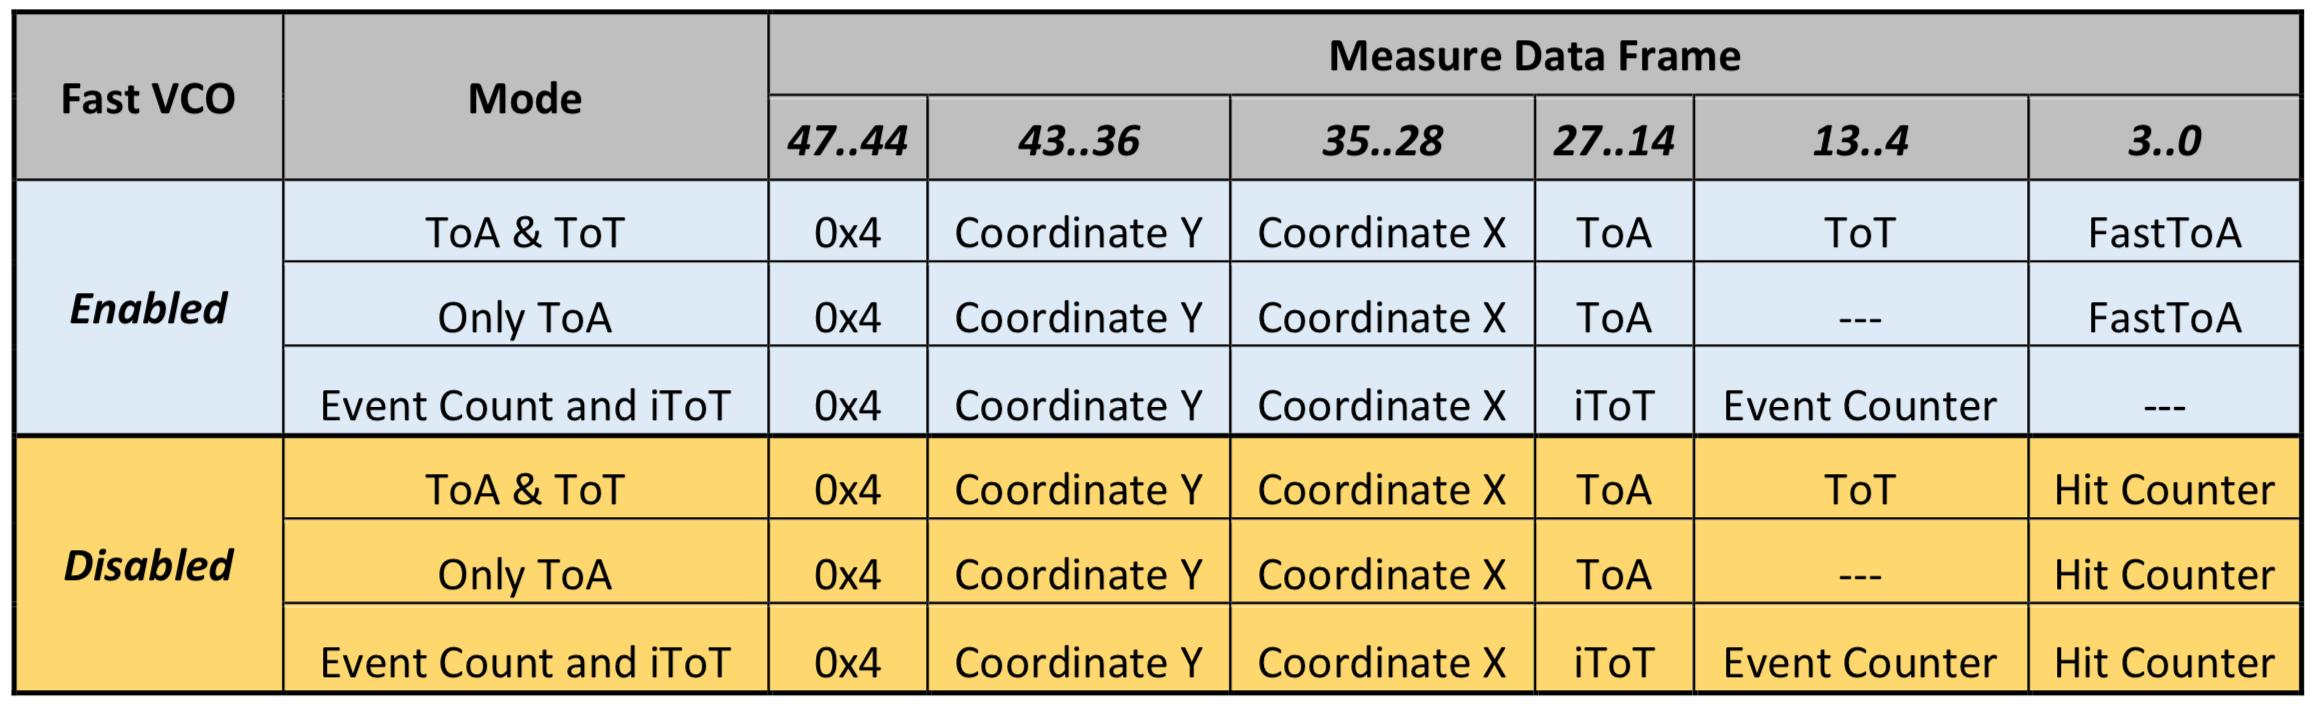
\includegraphics[width=14cm]{figures/katherine_pixel_measurement_data.png}
        \caption{Struktura měřených dat \cite{katherine_docs}.}
        \label{tab:katherine:protocol:measurement_data_structure}
    \end{center}
\end{table}

%********************************************************************************
% Komunikační modul
%********************************************************************************
\section{Komunikační modul}\label{chap:katherine:comm}
Pro účely řízení komunikačního rozhraní \textit{Katherine} a vyčítání měřených dat byl implementován komunikační modul, který bude popsán v této podkapitole. Aby bylo možné integrovat modul do systému, musí obsahovat implementaci komunikačního interface (viz \ref{chap:handler:detector_layer:commIntf}), které musí být v manifestu zkompilovaného \texttt{jar} archívu explicitně uvedeno (viz \ref{chap:handler:detector_layer:module_init}).

Na obrázku \ref{fig:katherine:comm:arch} je přehled vrstev softwarové architektury komunikačního modulu, které budou dále popsány v následujících podkapitolách.

\begin{figure}[h]
	\begin{center}
		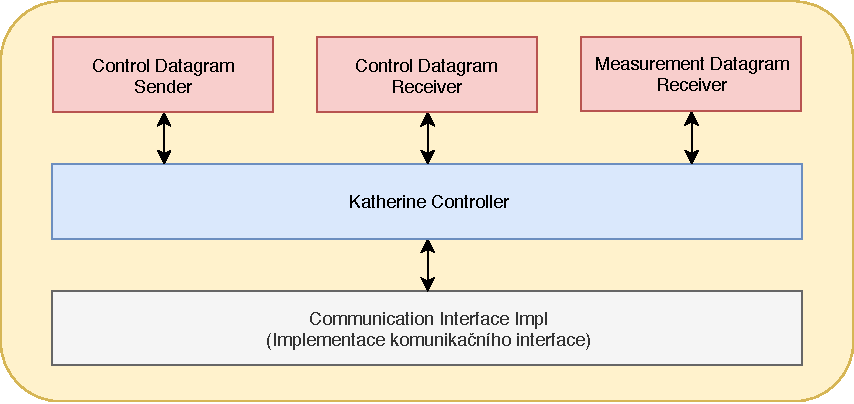
\includegraphics[width=14cm]{figures/katherine_comm_arch.pdf}
		\caption{Softwarová architektura komunikačního modulu, implementujícího komunikační interface.}
		\label{fig:katherine:comm:arch}
	\end{center}
\end{figure}

\subsection{Implementace komunikačního interface}
Tato vrstva slouží jako tzv. fasáda\footnote{Návrhový vzor fasáda (\textit{Facade Pattern}) - použití pro poskytování zjednodušeného interface pro komplexní části kódu (analogie s pojmem fasáda, známém z architektury).} Katherine kontroléru. Implementace komunikačního interface implementuje všechny jeho metody, vč. poskytování přehledu a podpory vykonávání \textit{ValueCommands} a \textit{ExecutionCommands} (pro jejich definici viz soubor \texttt{detector\_model.json} na přiloženém CD, viz příloha \ref{chap:app:cd}), navazování spojení s detektorem, nahrávání konfigurace apod.

Po zavedení modulu je vytvořena fronta měřených dat, která je přejatá handlerem.

Připojením detektoru vzniká instance Katherine kontroléru, dle předané konfigurace. Při odpojení detektoru je kontrolér notifikován, aby mohl uvolnit svoje prostředky (např. uzavřít síťové spojení) a poté je odstraněn.

\subsection{Katherine kontrolér}
Tato vrstva udržuje spojení s detektorem a implementuje všechny potřebné řídící příkazy detektoru.

Odesílání řídících příkazů je realizováno pomocí komponenty \texttt{Control Datagram Sender} (viz obr. \ref{fig:katherine:comm:arch}), který implementuje asynchronní frontu datagramů. Fronta je asynchronně zpracovávána nezávislým vláknem, které datagramy z fronty odesílá na řídící port \textit{Katherine}.

O příjem dat z řídícího socketu se stará komponenta \texttt{Control Datagram Receiver}, která v separátním vlákně přijímá příchozí data. Každý příchozí datagram (8-bytový vektor) je zpracován a přidán do fronty příchozích řídících dat. Komponenta také implementuje blokující metodu pro přijetí dat, která dle zadaného ID příkazu a maximálního času čekání (tzv. \textit{timeout}) hledá požadovanou odpověď ve frontě dat.

Příklad použití obou komponent zmíněných výše je ve zdrojovém kódu \ref{src:katherine:comm:example_get_bias}. Příklad demonstruje vyčtení biasu z detektoru. Nejprve je pomocí \texttt{Control Datagram Sender} odeslán řídící příkaz s ID 0x0C (řádek 3 až 7) a následně pomocí \texttt{Control Datagram Receiver}, resp. pomocí jeho blokující metody popsané výše, je zachycena odpověď, ze které je vyčtena požadovaná hodnota napětí. Jestli se odpověď nepodaří přijmout ve zvoleném timeoutu, je vygenerována výjimka, která musí být vyššími vrstvami programu ošetřena.

\begin{code}[h]
    \begin{minted}[
      frame=single,
        linenos,
        breaklines
      ]{Kotlin}
@Throws(DetectorException::class)
fun getBias(): Float {
    packetSender.send(
        PacketBuilder.builder()
            .commandID(KatherineValueCommands.BIAS.getterCommandId)
            .build()
    )

    val packet = packetReceiver.pollPacketFromQueue(
        KatherineValueCommands.BIAS.getterCommandId,
        RESPONSE_TIMEOUT
    )
    return packet.floatValue
}
    \end{minted}
    \caption{Příklad implementace řídícího příkazu \textit{Katherine} pro vyčtení biasu pomocí komponent \texttt{Control Datagram Sender} a \texttt{Control Datagram Receiver}.}
    \label{src:katherine:comm:example_get_bias}
\end{code}

Poslední komponentou je \texttt{Measurement Datagram Receiver}, který ve svém separátním vlákně přijímá příchozí datagramy na socketu pro detektorem měřená data, jejichž struktura už byla popsána v \ref{chap:katherine:protocol:measure_data_structure}. Každá příchozí událost je zpracována (identifikace hlavičky apod.) a vložena do fronty měřených dat, která je zpracovávána datovým modulem.

%********************************************************************************
% Datový modul
%********************************************************************************
\section{Datový modul}\label{chap:katherine:data}
Datový modul implementuje \texttt{DataPersistence} interface (viz \ref{chap:handler:detector_layer:dataIntf}). Po jeho zavedení do systému je mu handlerem předána fronta dat, kterou po spuštění začne zpracovávat.

Fronta dat obsahuje objekty, které jsou potomky objektu \texttt{AbstractDataFrame} (který je součástí modelu poskytovaných knihoven). V rámci modulu se společnou \textit{code-base} \textit{Katherine} modulů (viz úvod kapitoly \ref{chap:katherine}) byly implementovány tyto třídy, které jsou potomky třídy \texttt{AbstractDataFrame}:
\begin{description}
    \item[\texttt{DataFrame}] - třída obsahující jednu událost, přenesenou datovým socketem z \textit{Katherine} rozhraní. Objekt obsahuje dekódovanou hlavičku a vlastní data, dle typu datagramu - viz tabulka \ref{tab:katherine:protocol:data_packet_header}.
    \item[\texttt{ControlFrame}] - obsahuje informaci generovanou komunikačním modulem, např. o začátku nebo ukončení akvizice apod.
    \item[\texttt{AcqConfigurationFrame}] - instance tohoto objektu je poslána komunikačním modulem na začátku akvizice dat a obsahuje informace o stavu a konfiguraci detektoru (např. bias, vyčítací mód, teploty apod.).
\end{description}  

Výstupem datového modulu jsou soubory s jednotlivými měřeními ve formátu \texttt{ASCII}, které jsou ukládány do zvoleného adresáře dle konfigurace. Příklad obsahu takového souboru je uveden v příloze \ref{chap:app:katherine:data_example}. Všechny časové údaje jsou v \texttt{UTC} čase. Formát pojmenovávání souborů je \texttt{název\_detektoru\_yyyy\_MM\_dd-HH\_mm\_ss.txt}.

Rovněž byla implementována varianta datového modulu, který ukládá pořízená data do \textit{MongoDB} databáze (viz \ref{chap:arch:technologie:mongodb}).

%********************************************************************************
% Katherine emulátor
%********************************************************************************
\section{Katherine emulátor}\label{chap:katherine:emulator}
Pro účely vývoje a testování byl vyvinut emulátor, které emuluje funkci \textit{Katherine} vyčítacího rozhraním s připojeným \textit{Timepix3} (viz \ref{chap:detectors:medipix_overview:timepix3}) detektorem na síťové vrstvě. Byla implementována podpora pro všechny řídící příkazy uvedené v \ref{chap:katherine:protocol:control_commands}, které jsou relevantní k akvizici dat (tj. např. akviziční čas, akviziční mód, vyčítací mód, bias, počet snímků apod.) a také příkazy pro měření teplot, vyčítání ID senzoru, či provádění testu digitální částí detektoru. Emulátor rovněž podporuje všechny datagramy pro přenos měřených dat (viz \ref{chap:katherine:protocol:measure_data_structure}).

Emulátor byl vyvinut v jazyce \texttt{Java}, resp. \texttt{Kotlin} (viz \ref{chap:arch:technologie:kotlin}).

\subsection{Softwarová architektura}
Na obrázku \ref{fig:katherine:emulator:arch} jsou znázorněny jednotlivé komponenty emulátoru. Základním prvkem je jeho jádro (na obr. \ref{fig:katherine:emulator:arch} jako \textit{emulator core}), které je vytvořeno po spuštění emulátoru. Společně s jádrem je vytvořen také \textit{Control Datagram Receiver}, který přijímá příchozí datagramy na komunikačním socketu detektoru. Příchozí řídící datagram je dále zpracován dle jeho hlavičky a klientovi je odeslána příslušná odpověď.

\begin{figure}[h]
	\begin{center}
		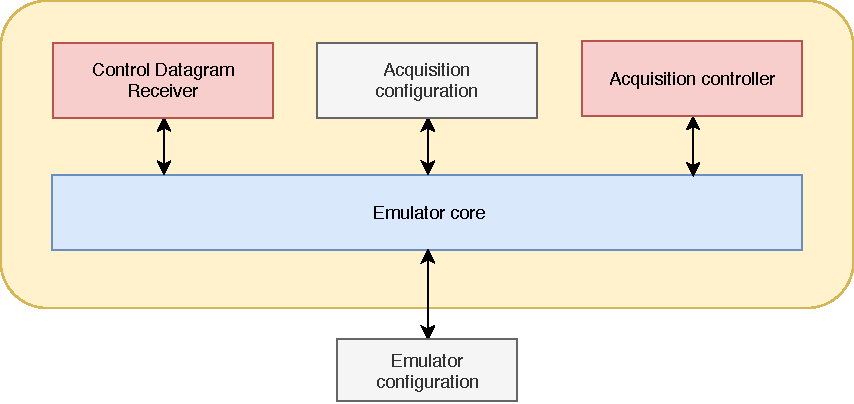
\includegraphics[width=14cm]{figures/katherine_emulator_arch.pdf}
		\caption{Softwarová architektura \textit{Katherine} emulátoru.}
		\label{fig:katherine:emulator:arch}
	\end{center}
\end{figure}

Z pohledu zpracování je možné příkazy rozdělit do tří kategorií:
\begin{description}
    \item[Nastavující akviziční parametry] - do této skupiny spadají všechny příkazy, které nastavují, nebo vracejí konfigurační parametry detektoru, jako je akviziční čas, bias, akviziční a vyčítací mód apod.
    \item[Řídící akvizici] - do této kategorie patří příkazy \textit{Acquisition Start} (0x03) a \textit{Acquisition Stop} (0x06). Po spuštění akvizice je vytvořena instance \texttt{Acquisition Controller}, který dle konfigurace začne generovat události a posílat je datovým socketem klientovi.
    
    Příkaz \textit{Acquisition Stop} pak přeruší probíhající akvizici.
    \item[Ostatní] - do této kategorie spadají ostatní příkazy, které nebyly zahrnuty v předchozích kategoriích (např. pro měření teploty, čtení \textit{chip id}, verze FW apod.).
\end{description}

Některé příkazy nebyly implementovány, protože simulace jejich funkce není triviální a je nad rámec požadované funkcionality (jsou to např. příkazy pro nastavování hodnot DAC, registrů apod.). Odpovědí na tyto příkazy bude vždy ACQ (viz \ref{chap:katherine:protocol:control_commands}).

\subsection{Konfigurace a nasazení}
Pro spuštění emulátoru vyčítacího rozhraní \textit{Katherine} je třeba mít nainstalované \texttt{JRE 8}\footnote{\textit{Java SE Runtime Environment, dostupné z\\\url{https://www.oracle.com/technetwork/java/javase/downloads}}.}, nebo vyšší.
Zkompilovanou java aplikaci je třeba spustit s argumentem cesty ke konfiguračnímu souboru (pro příklad viz zdrojový kód \ref{src:emulator:config}). Konfigurační soubor obsahuje číslo portu, na které bude emulátor naslouchat pro řídící příkazy (\texttt{portCommands}), číslo portu a adresu pro odesílání měřených dat (\textit{portCommands} a \texttt{hots}) a parametr udávající průměrný počet události, které budou v rámci jedné akvizice vygenerovány.

Aplikaci je tedy možné spustit například takto: \mint{bash}{java -jar emulator.jar config.yaml}

\begin{code}[h]
  \begin{minted}[
  frame=single,
  linenos,
  breaklines
  ]{yaml}
portCommands: 1555
portData: 1556
host: 127.0.0.1
avgNumberOfEventsPerAcq: 10
\end{minted}
\caption{\texttt{YAML} konfigurační soubor emulátoru vyčítacího rozhraní \textit{Katherine}.}
\label{src:emulator:config}
\end{code}